% По умолчанию используется шрифт 14 размера. Если нужен 12-й шрифт, уберите опцию [14pt]
%\documentclass[14pt]{matmex-diploma}
\documentclass[14pt]{matmex-diploma-custom}

\begin{document}
% Год, город, название университета и факультета предопределены,
% но можно и поменять.
% Если англоязычная титульная страница не нужна, то ее можно просто удалить.
\filltitle{ru}{
    chair              = {Программная инженерия\\Системное программирование},
    title              = {Исправление ошибок в зашумленных последовательностях при помощи графов сборки},
    % Здесь указывается тип работы. Возможные значения:
    %   coursework - Курсовая работа
    %   diploma - Диплом специалиста
    %   master - Диплом магистра
    %   bachelor - Диплом бакалавра
    type               = {master},
    position           = {студента},
    group              = 444,
    author             = {Клещин Антон Сергеевич},
    supervisorPosition = {доц. каф. СП, к. т. н.},
    supervisor         = {Литвинов Ю.\,В.},
    supervisorPositionx   = {доц. каф. стат. мод., к. ф.-м. н.},
    supervisorx           = {Коробейников А.\,И.},
    supervisorPositiony   = {старший н. с., к. ф.-м. н.},
    supervisory           = {Пржибельский А.\,Д.},
    reviewerPosition  = {приглашённый н. с., к. ф.-м. н.},
    reviewer          = {Нурк С.\,Ю.},
%   university         = {Санкт-Петербургский Государственный Университет},
%   faculty            = {Математико-механический факультет},
%   city               = {Санкт-Петербург},
%   year               = {2013}
}
\filltitle{en}{
    chair              = {Software and Administration of Information Systems \\ Software Engineering},
    title              = {Error correction in noisy sequences using assembly graphs},
    type               = {master},
    author             = {Anton Kleshchin},
    supervisorPosition = {C.Sc., Associate Professor},
    supervisor         = {Yurii Litvinov},
    supervisorPositionx   = {Ph.D., Associate Professor},
    supervisorx           = {Anton Korobeynikov},
    supervisorPositiony   = {Ph.D., Senior Research Fellow},
    supervisory           = {Andrey Prjibelski},
    reviewerPosition  = {Ph.D., Visiting Fellow},
    reviewer          = {Sergey Nurk},
}
\maketitle
\tableofcontents
\setcounter{secnumdepth}{4}
%==============================================================================
% У введения нет номера главы
\section*{Введение}
Сборка геномов является одной из важнейших задач биоинформатики. За многие годы учёным уже удалось собрать, а затем и расшифровать большое количество геномов. Несмотря на это, автоматическая реконструкция генома всё ещё остаётся сложной вычислительной задачей \cite{sohn2018present, art:collins2018challenge}.

Обычно сборка генома происходит из ридов (англ. reads) --- фрагментов ДНК, которые получаются в результате секвенирования, а результатом являются контиги (англ. contigs, восстановленные части ДНК из ридов) или скаффолды (англ. scaffolds, восстановленные части ДНК с пропусками известной длины).

Технологии секвенирования не стоят на месте: появилось третье поколение, позволяющие получать длинные риды дешевле, но количество ошибок в них на порядок выше \cite{art:reads}. Несмотря на то, что есть способы частично бороться с этими ошибками \cite{art:alic2016objective}, для улучшения результатов сборки можно прибегнуть к другим методам. Например, для небольших геномов активно применяется метод гибридной сборки \cite{art:hybridSpades}, в которой одновременно используются как длинные риды с большим количеством ошибок, так и короткие, уровень ошибок в которых минимален. Короткие риды здесь выступают основным материалом для построения графа сборки, а длинные риды позволяют находить более длинные пути в этом графе, которые в дальнейшем становятся контигами. К сожалению, для больших геномов получить достаточное количество коротких ридов оказывается очень дорого.

Кроме того, даже с небольшими геномами есть проблемы. Например, есть штаммы бактерий, получить большое количество экземпляров которых крайне сложно. В этом случае покрытие генома полученными ридами оказывается очень низким, как и качество длинных ридов. Более того, некоторые штаммы вообще невозможно получить без окружающих их бактерий, поэтому прибегают к метагеномике --- направлению геномики, в котором рассматриваются ДНК не отдельного организма, а сразу множества. Покрытие ридами генома каждой бактерии в рамках одной сборки может сильно отличаться, что только ухудшает качество контигов бактерий с низким покрытием.

Уже существуют инструменты, которые стараются исправлять контиги, используя риды. Их основная идея --- найти выравнивания ридов на контиги и с помощью какого-нибудь алгоритма консенсуса решить, какие нуклеотиды исправлять. При этом подходе теряется информация, которую нам даёт граф сборки. Во-первых, рёбра графа в основном существенно длиннее ридов, а также уже проведена коррекция ошибок в самих ридах. Во-вторых, граф сборки даёт связи между рёбрами. Так как любой контиг это путь в графе, то можно попытаться исправить фрагмент контига, найдя подходящий путь между рёбрами, в местоположении которых в контиге мы уверены.

Итак, оказывается актуальной разработка нового инструмента, позволяющего исправлять ошибки в контигах при помощи графов сборки.

%==============================================================================
\section{Постановка задачи}
Целью данной работы является создание инструмента, позволяющего исправлять ошибки в контигах при помощи графов сборки. Для достижения этой цели были сформулированы следующие задачи.
\begin{itemize}
    \item Формирование критериев фильтрации выравниваний рёбер графа на последовательности.
    \item Разработка алгоритма исправления ошибок за пределами выравненных рёбер.
    \item Разработка алгоритма переноса полученных путей в графе обратно в последовательности.
    \item Реализация итогового алгоритма в виде отдельного инструмента.
    \item Апробация алгоритма на известных геномах.
\end{itemize}

%==============================================================================
\section{Обзор предметной области}
\subsection{Представление генома}
Большинство природных ДНК состоит из двух скрученных спиралей, к которым крепятся молекулы, называемые нуклеотидами \cite{art:Watson}. Всего в спиралях присутствует четыре вида нуклеотида: аденин (A), цитозин (C), гуанин (G), тимин (T). Двойная спираль ДНК может иметь либо линейную структуру, либо кольцевую. Одноцепочечную ДНК содержат лишь некоторые вирусы и бактериофаги. При этом известно, что одна спираль полностью задаёт другую: напротив каждого нуклеотида из одной цепочки стоит комплементарный ей из другой. Для аденина это тимин, а для гуанина --- цитозин.

Таким образом можно считать, что ДНК состоит из двух комплементарных строк над алфавитом из четырёх букв. Длину подстрок принято измерять в спаренных основаниях (англ. base pair, \textbf{bp}), которые эквивалентны одному символу строки.

\subsection{Секвенирование и сборка геномов}
Современные технологии не могут считывать всю ДНК за раз, поэтому в результате секвенирования получается множество фрагментов ДНК, называемых ридами. В зависимости от используемой технологии, длины ридов можно разделить на два класса: короткие и длинные. Короткие риды получают, в основном, при использовании технологии Illumina \cite{art:reads}, которая получает цепочки нуклеотидов порядка 100-200 bp. Длинные риды получают технологиями Pacbio и Oxford Nanopore \cite{art:reads}, которые получают цепочки порядка 10 и 100 kpb соответственно. Для сравнения, например, длина генома у бактерий измеряется в миллионах bp, у простых многоклеточных в сотнях миллионов bp, а у человека геном содержит около три миллиардов нуклеотидов.

К сожалению, при секвенировании происходят ошибки, поэтому ДНК читается несколько раз, чтобы в покрытии каждого нуклеотида результирующим набором ридов было больше правильных значений, чем ошибочных. В коротких ридах уровень ошибок составляет около 0.1-1\%, в то время как для длинных ридов это значение доходит до 10-15\% \cite{art:reads}.

Задачей ассемблера является восстановление одной из нитей спирали ДНК по ридам. Обычно удаётся  восстановить лишь фрагменты ДНК, которые являются либо контигами, либо скаффолдами. Их отличие в том, что в случае скаффолдов допускаются подстроки, в которых нуклеотиды неизвестны, что даёт дополнительную информацию в виде расстояния между контигами и их порядка следования в геноме.

Так как в коротких ридах мало ошибок, то достаточно небольшого покрытия генома ридами, чтобы граф, а следовательно и контиги, практически не содержали ошибки. Для длинных же ридов для достижения такого же результата покрытие должно быть большим, что иногда бывает просто невозможно получить, и к тому же дополнительные эксперименты стоят очень дорого.

\subsection{Граф сборки}
Методы сборки ридов в контиги далеко шагнули вперёд. В некоторых современных ассемблерах, таких как SPAdes \cite{art:SPAdes} и Flye \cite{art:flye}, используется подход, основанный на графе де Брюйна (англ. de Bruijn graph) \cite{art:Pevzner}. Этот граф строится по следующим принципам: берётся набор входных строк и выделяется из них множество всевозможных подстрок длины k+1 (k+1-меры). Тогда направленными рёбрами будут выступать k+1-меры. Вершинами же будут k-меры, полученные уже из k+1-меров и выступающие в роли перекрытия между ними. Соответственно, к вершине подсоединяются рёбра тем концом, который содержит k-мер вершины. Пример графа можно видеть на рисунке \ref{fig:debruijn}.

\begin{figure}[h]
	\centering
	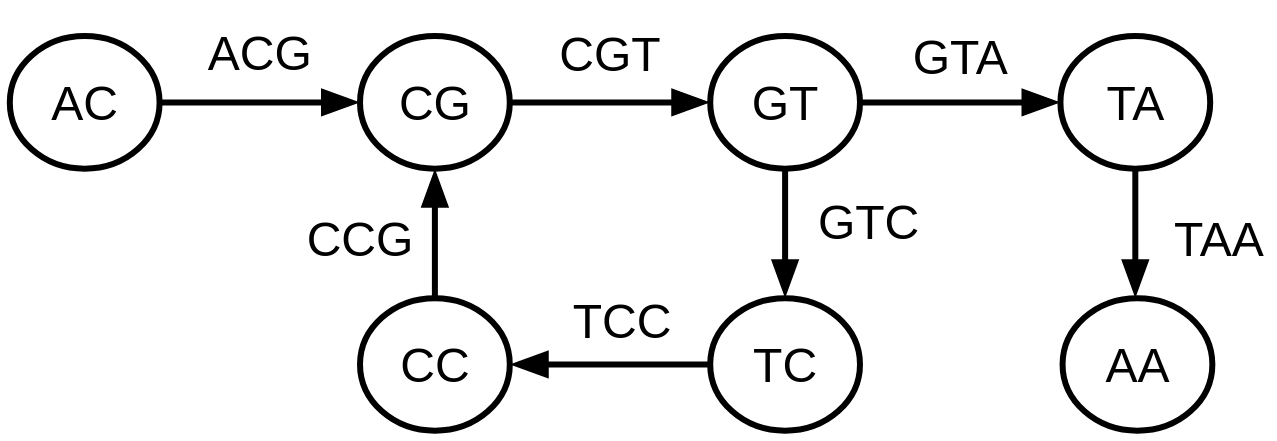
\includegraphics[scale=0.3]{debruijn.png}
	\caption{Граф де Брюйна для строки ACGTCCGTAA с параметром ${k=2}$.}
	\label{fig:debruijn}
\end{figure}

Максимальное количество возможных вершин в графе де Брюйна равно $4^k$, а количество рёбер между ними --- $4^{k+1}$. При небольших значениях $k$ в графе, скорее всего, будут присутствовать почти все варианты вершин, а сам граф будет близок к полносвязному, что даёт плохое представление о геноме. С другой стороны, при больших $k$ граф может распасться на несвязные компоненты. Поэтому, например, ассемблер SPAdes проводит последовательно несколько сборок для разных $k$ и часто останавливается для запутанных геномов и метагеномов на значении 55.

Так как пути в графе де Брюйна образуют контиги, вершины, в которые входит и выходит ровно по одному ребру, можно удалить, объединив соответствующие рёбра в одно. Пример такого упрощения можно видеть на рисунке \ref{fig:debruijn_simpl}.

\begin{figure}[h]
	\centering
	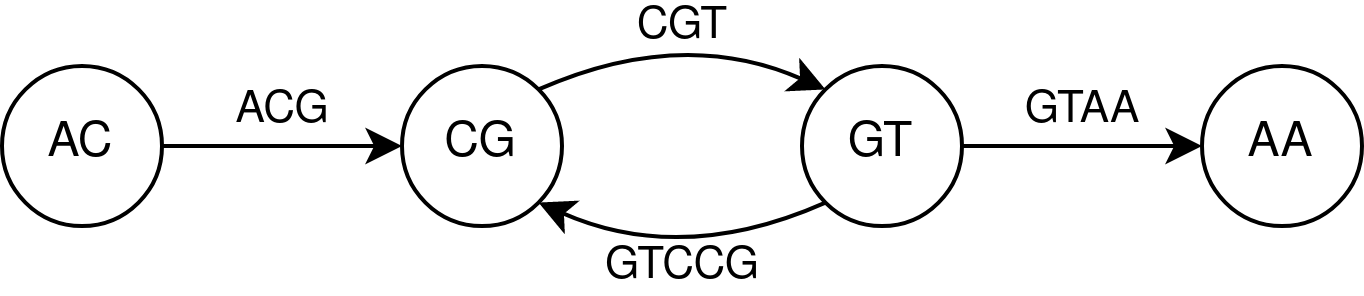
\includegraphics[scale=0.22]{debruijn_simpl.png}
	\caption{Граф сборки, полученный в результате упрощения графа с рисунка \ref{fig:debruijn}.}
	\label{fig:debruijn_simpl}
\end{figure}

Граф, полученный в результате упрощения графа де Брюйна, называется графом сборки. На самом деле, упрощение необходимо по нескольким причинам, которые описаны в работе \cite{art:disser_andrey}. В частности, это позволяет удалить рёбра, в которых содержатся ошибки.

\subsection{Выравнивание последовательностей}
Выравнивание последовательностей --- это процесс сопоставления символов одной строки символам другой так, чтобы чтобы максимизировать функцию похожести этих последовательностей. Если мы ожидаем, что последовательности небольшие и должны хорошо совпадать по всех свой длине, то в качестве функции похожести можно взять редакционное расстояние. Если известны какие-то особенности последовательностей, то лучше воспользоваться аффинным выравниванием (например, можно не штрафовать за большие несовпадающие участки). Находить точное значение функции требует количество действий, пропорциональное произведению длин, что для длинных строк неприемлемо, поэтому ограничиваются лишь приближёнными значениями.

Особенностью выравнивания ребер графа сборки на последовательность заключается в том, что ребро может соответствовать одновременно нескольким фрагментам последовательности, а также выравниваться лишь частично.

Помимо этого, существует задача выравнивания последовательности на целый граф сборки. В ней требуется найти \textit{путь} в графе, строковое представление которого максимально похоже на выравниваемую последовательность. 

\subsection{Инструменты для выравнивания последовательностей }

% \textbf{blat}

% \textbf{bwa}

\textbf{minimap2} \cite{art:minimap2} разрабатывался в ответ на появление технологий секвенирования, которые создают очень длинные риды (100 kbp в среднем). Его главное преимущество --- выравнивание длинных последовательностей DNA на большие референсные геномы более чем в 30 раз быстрее \cite{art:minimap2} по сравнению с существующими инструментами, при этом сохраняя достаточно высокий уровень точности.

\textbf{winnowmap} \cite{art:winnowmap} основывается на minimap2 и рассматривет проблему неравномерного распределения k-меров в геноме, уменьшая количество ложно-положительных совпадений. Однако впоследствии его идеи были включены в последние версии minimap2.

\textbf{GraphAligner} \cite{art:rautiainen2020graphaligner} основывается на идее выравнивание последовательности на граф на основе битового параллелизма \cite{art:bpstga}. Основное преимущество --- выравнивание в 12 раз быстрее и в 2 раза точнее по сравнению с существующими инструментами \cite{art:rautiainen2020graphaligner}. Помимо этого, полезной возможностью является нахождения не одного лучшего выравнивания, а сразу нескольких.

% \textbf{SPAligner} \cite{art:spaligner} основывается 

\subsection{Существующие решения}
\textbf{LoRDEC} \cite{art:salmela2014lordec} был первым, кто использовал граф де Брюйна, построенный из коротких ридов, в качестве индекса для исправления длинных ридов. В LoRDEC длинные риды привязывались к графу, используя общие k-меры. Затем непривязанные подпоследовательности исправлялись с помощью путей, которые похожи на исправляемые подпоследовательности. Многие инструменты для гибридного исправления ошибок в длинных ридах основываются на этом подходе LoRDEC.

\textbf{Jabba} \cite{art:miclotte2016jabba}, помимо использования подхода LoRDEC, перед построением графа применяет самокоррекцию коротких ридов. Кроме этого, длинные риды привязываются к графу, используя максимально точные совпадения, чтобы использовать k-меры разной длины во время исправления ошибок.

\textbf{HG-CoLoR} \cite{art:morisse2018hybrid} также применяет самокоррекцию коротких ридов, а также выравнивает их на длинные риды, чтобы найти перекрытия между собой. Эти перекрытия привязывают риды к графу де Брюйна переменного порядка с учётом разных длин k-меров.

\textbf{FMLRC} \cite{art:wang2018fmlrc} индексирует граф де Брюйна, используя многострочное преобразование Барроуза — Уилера (англ. multi-string Burrows-Wheeler Transform) коротких ридов. Это представление занимает мало места в памяти, допускает несколько длин k-меров и неявно сохраняет частоту появления k-меров. Исправление ошибок в FMLRC происходит в два прохода: во время первого используется небольшое значение k для k-меров, в то время как для второго используется k больше, чтобы упростить граф в особо сложных местах.

\textbf{CoLoRMap} \cite{art:haghshenas2016colormap}, в отличии от вышеупомянутых инструментов, строит граф взвешенных выравниваний из сопоставления коротких ридов длинным. Это сопоставление позволяет получить пути в графе, которые максимально похожи на подпоследовательности исправляемых последовательностей. CoLoRMap использует информацию о парных концах коротких ридов, чтобы перепрыгнуть регионы длинных ридов, которым не сопоставлен ни один короткий рид.

\textbf{Ratatosk} \cite{art:holley2021ratatosk} в свою очередь, во первых, раскрашивает вершины графа де Брюйна с помощью коротких и длинных ридов, чтобы выделить существующие пути для исправления. Раскраска графа позволяет уменьшить пространство обхода графа, удаляя химерные пути.
Во вторых, длинные риды привязываются к графу, используя как точное совпадение k-меров, так и неточное, что позволяет привязать регионы с большим количеством ошибок. В третьих, граф аннотируется кандидатами на точечные ошибки в один нуклеотид, что позволяет выделить небольшие вариации между гаплотипами, которые трудно уловить из ошибочных длинных ридов. В четвёртых, коррекция выполняется в два прохода, используя короткие и длинные риды по отдельности.

Для получения большей информации об исправлении ошибок в длинных ридах можно воспользоваться обзорами \cite{art:morisse2020long, art:zook2016extensive, art:zhang2020comprehensive}.

\subsection{Оценка качества сборки}
Для того чтобы понять, насколько результат сборки соответствует реальному геному, существует много метрик. Одни можно вычислить только по результату сборки, другие же требуют наличие референсного генома --- некоторого эталонного генома для данного вида организма. Метрики, использующие референсный геном, позволяют намного детальнее оценить качество сборки. Стоит отметить, что собранный геном не должен полностью совпадать с референсным геномом, так как геном исследуемого организма может отличаться от эталонного на 1-2\%.

Одной из программ, позволяющих вычислять оба вида метрик, является QUAST \cite{art:QUAST}. Помимо одиночных геномов он также поддерживает использование  метагеномов для оценки качества сборки как отдельных геномов в него входящих, так и их объединения \cite{art:metaquast}.

%==============================================================================
\section{[TODO: fix constants uses] Алгоритм}

Представленный в данной работе алгоритм является эвристическим. Все приведённые точные значения являются параметрами алгоритма по-умолчанию и были получены как оптимальные при тестировании на различных данных.

\begin{figure}[h]
    \centering
\begin{tikzpicture}[
    every node/.style={
      draw=black,
      anchor=west,
      minimum height=1cm,
      rounded corners 
      }, 
    font=\small
    ]
    \begin{scope}[on grid]
    \node[ellipse, inner sep=0pt] (graph)               {граф сборки};
    \node (align) [left = 2cm of graph.west] {1. выравнивание рёбер графа на последовательности};
    \node[draw=purple] (filter) [below  right = 2cm and 7cm of align] {2. фильтрация выравниваний};
    \node[draw=purple, align=left] (filling) [below = 2cm of filter] {3. нахождение и смешивание путей \\ между выравниваниями};
    \node[draw=purple] (write back) [left = 1cm of filling.west] {4. перенос путей в последовательности};
    \node[ellipse, inner sep=0pt] (seq)  [above = 2cm of write back] {зашумлённые последовательности};
    \end{scope}

    \path[->]
    (align) edge (filter)
    (filter) edge (filling)
    (filling) edge (write back)
    ;
    \path[->, dashed]
    (graph) edge (align) edge [bend left=54] (filling)
    (seq) edge (align) edge (filling) edge (write back)
    ;
\end{tikzpicture}
\caption{Алгоритм коррекции. Фиолетовым цветом обозначены стадии, описанные в данной работе. Пунктирными стрелочками --- использование данных.}
\label{fig:pipeline}
\end{figure}

Алгоритм коррекции состоит из следующей последовательности шагов, изображённых на рисунке \ref{fig:pipeline}.
\begin{enumerate}
    \item Рёбра графа сборки выравниваются на исправляемые последовательности с помощью какого-нибудь выравнивателя. Так как в графе уже присутствуют как прямые рёбра, так и обратно-комплементарные, необходимо получить выравнивания рёбер только в их прямом направлении. Кроме того, так как в графе есть неуникальные рёбра (например, отражают повтор в геноме или принадлежат нескольким организмам в метагеноме), необходимо получить все выравнивания ребра, которые нашёл выравниватель, а не только одно наилучшее.
    \item Найденных выравниваний довольно много, они перекрывают друг друга, и далеко не все из них действительно должны находиться на найденных местах (например, повторы). Поэтому их нужно отфильтровать. Те выравнивания рёбер, что останутся, будем называть \textit{якорями}.
    \item Помимо исправления последовательностей непосредственно якорями, нужно исправлять и другие места. Для этого между якорями находятся пути, которые затем смешиваются для получения строки, которая заменит фрагмент последовательности между этими якорями. Будем называть такие строки \textit{строками-заменителями}. Якоря со строками-заменителями между ними образуют \textit{смешанный путь} в графе.
    \item Полученные смешанные пути переносятся в исправляемые последовательности.
\end{enumerate}

\subsection{Выбор якорей}
Из множества всех найденных выравниваний на рёбра графа нас интересуют те, которые ``скорее всего'' находятся на правильном месте. Так, например, с увеличением длины ребра, вероятность, что оно будет выравнено на множество мест, уменьшается.

Для выбора якорей используются два фильтра: грубый (англ. rough) и точный (англ. fine). Грубый фильтр работает на этапе чтения выравниваний и оценивает их правильность в отрыве от остальных выравниваний посредством следующих критериев:
\begin{itemize}
    \item длина выравнивания (а значит и длина ребра) больше минимальной разрешённой длины ($300$ символов);
    \item выравненные фрагмент последовательности и фрагмента ребра совпадают хотя бы на половину, то есть их идентичность\footnote{Отношение удвоенного количества совпавших символов к сумме длин сопоставленных подстрок.} (англ. identity) $> 50\%$;
    \item разница длин выравненных фрагмента последовательности и фрагмента ребра не превышает ожидаемого уровня ошибочности сборки, что на практике бывает около $5\%$;
    \item выравнивание является одним из случаев:
    \begin{itemize}
        \item ребро полностью содержится в последовательности;
        \item последовательность полностью содержится в ребре;
        \item конец ребра является началом последовательности;
        \item начало ребра является концом последовательности\footnote{Часто ``конец/начало ребра/последовательности'' не является суффиксом/префиксом из-за наличия ошибок, поэтому необходимо допускать небольшой отступ, например, не больше $k$ символов.};
        \item выравнялась лишь часть ребра, но она достаточно длинная ($\ge 2000$ символов), чтобы можно было считать это структурным отличием графа от последовательности;
    \end{itemize}
\end{itemize}

Точный фильтр оценивает правильность выравнивания на основе уникальности. Выравнивание считается \textit{уникальным}, если его ребро имеет не больше одного выравнивания, которое полностью содержится в какой-либо последовательности. Выравнивание принимается точным фильтром, если оно:
\begin{itemize}
    \item длинное и уникальное;
    \item короткое, уникальное и идентичность выше $70\%$.
    \item неуникально и идентичность выше $90\%$.
\end{itemize}

Оставшиеся после фильтрации выравнивания рёбер будем называть \textit{якорями}. 

Для каждого якоря определяется уровень достоверности:
\begin{enumerate}
    \item высокий: якорь уникальный;
    \item средний: якорь неуникальный и средней длины ($\ge 1000$ символов);
    \item низкий: оставшиеся якоря;
\end{enumerate}

После фильтрации якоря потенциально всё ещё могут быть взаимоисключающими (то есть пересекаться больше, чем на $k$\footnote{Количество символов пересечения смежных рёбер в графе}$+\varepsilon$\footnote{Несколько символов для возможных ошибок, например, $5$}). Взаимоисключающие рёбра отбрасываются следующим образом:
\begin{itemize}
    \item для каждой пары якорей проверяется, конфликтуют ли они. Если да, то:
    \begin{itemize}
        \item если у них разные уровни достоверности, то на удаление помечается тот, что с меньшим;
        \item если уровни достоверности одинаковые и длины якорей отличаются больше, чем в два раза, то помечается тот, что с меньшей;
        \item иначе помечаются оба;
    \end{itemize}
    \item все помеченные якоря разом отбрасываются;
\end{itemize}

Тем не менее, критериев фильтрации на практике оказывается достаточно, чтобы взаимоисключающих рёбер было не больше всего нескольких единиц из класса с низким уровнем достоверности.

\subsection{Пути между якорями}
Расположим якоря в порядке встречи их в последовательности. Заполнение пространства вне якорей проходит следующим образом.
\begin{itemize}
    \item Для каждой пары смежных якорей самого достоверного класса находятся пути в графе, которые отличаются не больше, чем на $10\%$ от длины фрагмента последовательности между этими якорями. Найденные пути затем и смешиваются и формируют строки-заменители.
    \item Если между двумя якорями не было сформировано строк-заменителей, то в этот промежуток добавляются якоря из следующего класса достоверности и процесс поиска-смешивания-формирования повторяется.
\end{itemize}

Между якорями ищутся все пути, чтобы на этапе смешивания быть уверенным, что различия между гаплотипами не будут потеряны. Так как графы устроены довольно сложно, путей даже между не очень удалёнными якорями (несколько тысяч символов) может быть чрезвычайно много (десятки и сотни тысяч), то поиск имеет несколько ограничений, выход за которые, как показывает наша практика, не имеет смысла. Сам поиск проходит в два этапа.
\begin{enumerate}
    \item С помощью алгоритма Дейкстры в графе помечаются все вершины, через которые существует путь с заданным ограничением сверху на длину. Количество найденных вершин не должно превышать 3000.
    \item Поиском в глубину по помеченным вершинам выбираются все пути с заданными ограничениями на длину. При этом суммарное количество рекурсивных вызовов не должно превышать 3000, а если оно превысило 500, то дополнительно проверяется, чтобы в найденном пути было не больше 5 одинаковых рёбер.
\end{enumerate}
Если поиск обнаружил превышение данных ограничений, процесс получения строки-заполнителя между текущей парой якорей прерывается. Эти ограничения выбраны таким образом, чтобы большинство случаев поиска завершалось с большим запасом до их превышения, но на слишком запутанных частях графа они быстро прерывались.

\subsection{Смешивание путей}
После того, как все пути между якорями найдены, необходимо понять, что из этого может исправить последовательность, а что испортить. 
Для этого каждый путь выравнивается на фрагмент последовательности. Если расстояние между ними слишком велико, то этот путь отбрасывается. Часть с выравниванием является самой трудоёмкой частью всего пайплайна коррекции и занимает больше $95\%$ времени, поэтому происходит параллельно.

Оставшиеся пути упорядочиваются в порядке возрастания расстояния. Если остался всего один путь, или у первого пути расстояние существенно\footnote{Довольно часто лучшие пути имеют расстояние 0-5, что является несущественным отличием, чтобы однозначно сказать, что какой-то путь лучше. Поэтому, помимо процентного соотношения (в два раза), стоит использовать и абсолютный порог (на десять).} меньше, чем у второго, то этот путь становится \textit{кандидатом} на строку-заменитель.

Не каждый кандидат становится строкой-заменителем. Чтобы это произошло, он должен отличаться от фрагмента последовательности не больше, чем среднее количество ошибок в текущей последовательности (это значение вычисляется после выбора якорей на основании их среднего значения идентичности).

Довольно часто все найденные пути являются порождением подграфа, который представляет из себя набор ``пузырей'' (альтернатив из двух подпутей), например, как на рисунке \ref{fig:buldges}. 

\begin{figure}[h]
    \centering
    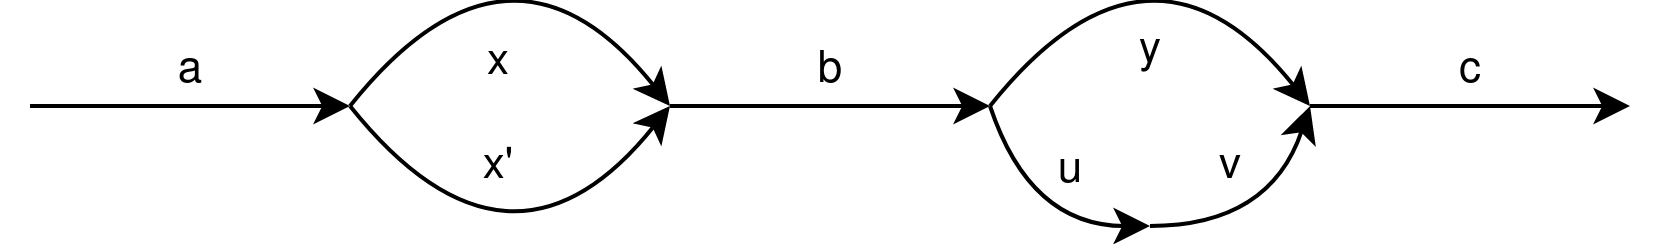
\includegraphics[width=0.95\textwidth]{buldges.png}
    \caption{Подграф, содержащий два ``пузыря'': (x, x') и (y, uv).}
    \label{fig:buldges}
\end{figure}

Пузыри зачастую образуются в результате наличия повторов в геноме, или когда есть похожие фрагменты у двух организмов (например, двух штаммах бактерии) в метагеноме. Рёбра в них отличаются весьма слабо, поэтому, если разложить такой подграф на два пути (с рисунка \ref{fig:buldges} это $axbyc$ и $ax'buvc$), можно выравнять эти пути между собой, найти места, которые в них отличаются, и заменить их на фрагменты из исправляемой последовательности. Таким образом вариации между гаплотипами будут сохранены, а ошибки исправлены. Полученная строка является также лишь кандидатом на строку-заменитель, чтобы избежать случайного внесения большого количества ошибок в последовательность.

Попытка сжатие пути до двух происходит следующим образом.  Сначала строится вспомогательный ориентированный граф. Для этого каждое ребро каждого пути представляются парой: id ребра и порядковый номер его вхождения в этот путь. Эти пары становятся вершинами в новом графе. Если два ребра стоят подряд в пути, то в новом графе между соответствующими им парами будет ребро. Пример на рисунке \ref{fig:compresed_paths}.

\begin{figure}[h]
    \centering
\begin{tikzpicture}[every node/.style={circle,draw=black}]
    \begin{scope}[on grid]
    \node (a0)               {$a,0$};
    \node (x)  [below right=1cm and 2.25cm of a0] {$x,0$};
    \node (y)  [right=2.5cm of x ] {$y,0$};
    \node (b)  [above right=1cm and 3.5cm of a0] {$b,0$};
    \node (a1) [above right=1cm and 2.25cm of y]  {$a,1$};
    \node (g0) [above right=1cm and 2.25cm of a1] {$g,0$};
    \node (g1) [right=2.5cm of g0] {$g,1$};
    \node (c)  [below right=1cm and 3.5cm of a1] {$c,0$};
    \node (d)  [below right=1cm and 2.25cm of g1] {$d,0$};
    \end{scope}

    \path[->]
    (a0) edge (b) edge (x)
    (b) edge (a1)
    (x) edge (y)
    (y) edge (a1)
    (a1) edge (g0) edge (c)
    (g0) edge (g1)
    (g1) edge (d)
    (c) edge (d)
    ;
\end{tikzpicture}
\caption{Пример сжатия четырёх путей (каждая буква является ребром пути): $abacd$, $abaggd$, $axyacd$, $axyaggd$. Первый путь даёт вершины $(a,0)$, $(b,0)$, $(a,1)$, $(c,0)$, $(d,0)$ и соединения между ними. Для остальных путей аналогично.}
\label{fig:compresed_paths}
\end{figure}

При и после построения вспомогательного графа проверяется его корректность: 
\begin{itemize}
    \item нет циклов и петель;
    \item начальные и конечные вершины совпадают с начальными и конечными вершинами каждого из путей;
    \item у каждой общей вершины не больше двух входящих и двух исходящих рёбер;
    \item у каждой вершины из альтернатив ровно по одному входящему и исходящему ребру;
\end{itemize}

Если граф получился корректным, то получаем два пути: первый состоит из общих вершин и первых альтернатив, а второй --- из общих вершин и вторых альтернатив. Если же корректность нарушена, то сжать пути не удалось и между текущими двумя якорями последовательность исправлена не будет.

Несмотря на то, что есть примеры, когда пути сжать можно, но он этого не делает (например, $aaa$ и $aba$), на практике этого алгоритма достаточно, чтобы сжать почти все подходящие наборы путей.

\subsection{Перенос путей в последовательность}
После того, как будут получены строки-заменители, их необходимо разместить обратно в исправляемую последовательность. Для определения фрагмента последовательности, соответствующего данной строке, используются выравнивания с первого шага алгоритма --- это диапазон с позиции первого символа первого якоря в составе строки до позиции последнего символа в последнем якоре в составе строки. Стоит отметить, что диапазоны строк-заменителей могут пересекаться вплоть до $k+\varepsilon$, при этом символы в перекрытии могут не совпадать. Чтобы избежать внесения ошибок, эти конфликты решаются следующим образом. Обозначим за $a$ и $b$ фрагменты перекрытия, соответствующие первой и второй строкам-заменителям, а за $s$ соответствующий фрагмент последовательности. Тогда:
\begin{enumerate}
    \item если $a=b$, то выбирается $a$;
    \item если $a=s$ или $b=s$, то выбирается $s$;
    \item в противном случае также выбирается $s$;
\end{enumerate}
Для 3его случая можно воспользоваться смешиванием из предыдущего шага, тем самым исправляя общие символы и не меняя несовпадающие, но на практике таких случаев обычно всего несколько штук на сборку, поэтому если ошибки и останутся неисправленным, то в пренебрежимо малом количестве.

\subsection{[TODO] Архитектура решения}


%==============================================================================
\section{Альтернативный алгоритм}
Можно заметить, что решение довольно похоже на решение задачи выравнивания последовательностей на граф (т.е. нахождение как можно более длинных путей в графе, которые соответствуют фрагментам последовательностей). Кажется, что отличие лишь в том, что мы дополнительно по-умному смешиваем пути между якорями на уровне нуклеотидов. Рассмотрим альтернативный алгоритм:
\begin{enumerate}
    \item взять существующий выравниватель на граф;
    \item взять несколько лучших выравниваний для каждого фрагмента последовательности;
    \item смешать найденные пути;
\end{enumerate}

\subsection{Кластеризация}
\begin{sloppypar}
Для проверки данного алгоритма был взят выравниватель GraphAligner. Он уже выдаёт несколько лучших найденных выравниваний для каждой области последовательности. Так как пути покрывают похожие, но не идентичные фрагменты, нужно разбить пути на кластера, которые будут покрывать как можно больше длины последовательности, и как можно меньше пересекаться (т.е. конфликтовать) друг с другом. Для этого будем последовательно объединять пути в кластера по следующему критерию: если два пути перекрываются выравниваниями больше, чем на $70\%$, то они лежат в одном кластере. Как показывает практика, на наших тестах этого критерия было достаточно, чтобы лучшие по идентичности пути в кластерах покрывали последовательность на $95-100\%$, все пути в кластере попарно пересекались минимум на $70\%$, а пути различных кластеров практически не пересекались ($<1\%$).
\end{sloppypar}

\subsection{Смешивание}
Пути в полученных кластерах смешиваются следующим образом.
\begin{enumerate}
    \item Выбирается лучший путь в кластере по идентичности с последовательностью.
    \item Все остальные пути выравниваются на лучший.
    \item По полученным выравниваниям помечаем символы и позиции между символами лучшего пути помечаются недостоверными, если хотя бы в одном выравнивании есть отличие.
    \item Недостоверные места заменяются символами из последовательности.
\end{enumerate}

Полученные после смешения строки переносятся обратно способом, описанным главе ``Перенос путей в последовательность''.

%==============================================================================

\section{Апробация}
В данной главе будет приведён сравнительный анализ реализации описанного в даной работе алгоритма на синтетических и настоящих метагеномах как с существующими решениями, так и с альтернативным алгоритмом.

\subsection{Метрики}
Сравнение качества коррекции начинается с выравнивания исправленных последовательностей на референсный геном. После этого для общих фрагментов используются следующие метрики:
\begin{itemize}
    \item \textit{количество замен} --- количество \textbf{символов} в выравнивании, в которых нуклеотиды последовательности не совпадают с сопоставленными им нуклеотидами референсного генома;
    \item \textit{количество вставок и удалений} --- количество \textbf{непрерывных участков} в выравнивании, которые присутствуют либо только в последовательностях, либо только в выравненной части референсного геноме;
    \item \textit{количество замен на 100 kbp} --- среднее количество замен на 100 kbp;
    \item \textit{количество вставок и удалений на 100 kbp} --- среднее количество вставок и удалений на 100 kbp;
    \item \textit{покрытие генома} --- процент нуклеотидов референсного генома, которые покрыты контигами;
    \item \textit{количество структурных ошибок} --- количество релокаций, инверсий, транслокаций. Пример изображён на рисунке \ref{fig:miss};
\end{itemize}

\begin{figure}[h]
    \centering
    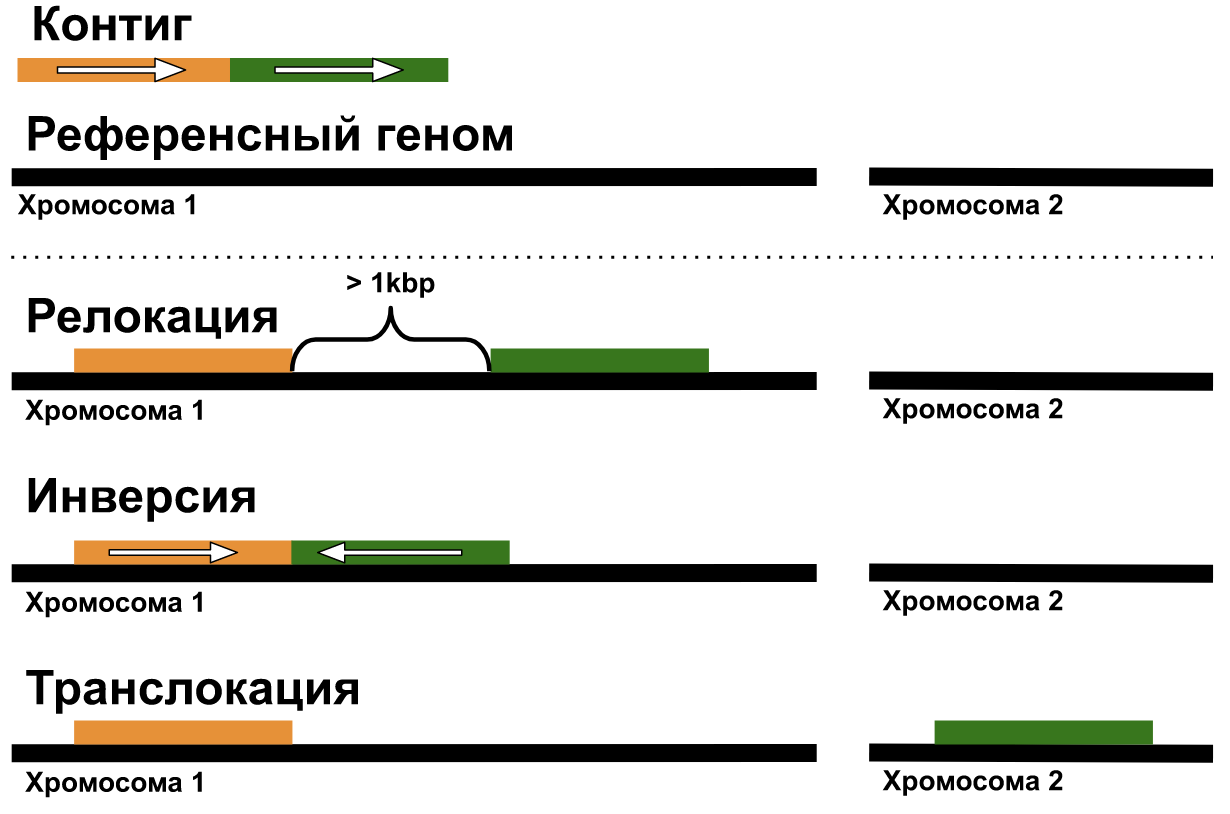
\includegraphics[scale=0.4]{misassemblies.png}
    \caption{Дан контиг, состоящий из двух частей, расположение которых при сопоставлении с референсным геномом определяет тип структурной ошибки.}
    \label{fig:miss}
\end{figure}

\begin{figure}[h]
    \centering
    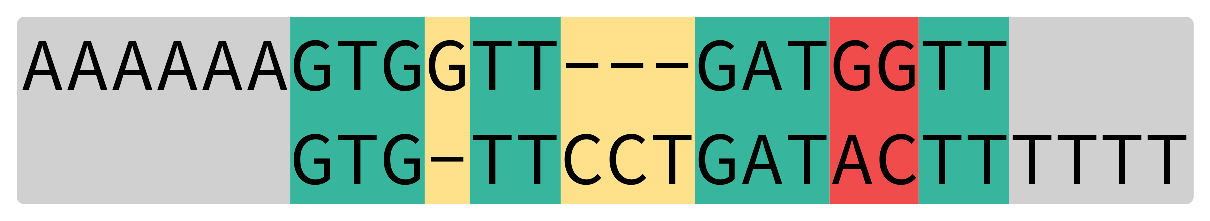
\includegraphics[width=0.7\textwidth]{alignment.eps}
    \caption{Пример выравнивания строк AAAAAAGTGGTTGATGGTT и GTGTTCCTGATACTTTTTT. Серым цветом выделены невыравненные фрагменты. Зелёным --- совпавшие фрагменты. Красным --- замены. Жёлтым --- вставки и удаления. }
    \label{fig:alignment}
\end{figure}

\subsection{[TODO] Схема сравнения}
На рисунке \ref{fig:common_pipeline} показана общая схема проведения сборки раздельно из длинных и коротких ридов.

\begin{figure}[h]
    \centering
\begin{tikzpicture}[
    every node/.style={
      draw=black,
      anchor=west,
      minimum height=1cm,
      align=center,
      rounded corners 
      }, 
    font=\small
    ]
    \begin{scope}[on grid]

        \node (cor1) {коррекция длинных\\ридов};
        \node (assembly) [right = 1cm of cor1.east] {сборка из длинных\\ридов};
        \node (cor2) [right = 1cm of assembly.east] {коррекция контигов сборки\\из длинных ридов};
        \node[ellipse, inner sep=0pt] (long reads) [above = 2cm of cor1] {длинные риды};
        \node[ellipse, inner sep=0pt] (graph) [above right = 2cm and 2cm of assembly] {граф сборки из коротких ридов};

    \end{scope}

    \path[->]
    (cor1) edge (assembly)
    (assembly) edge (cor2)
    ;
    \path[->, dashed]
    (long reads) edge (cor1)
    (graph) edge (cor1) edge (cor2)
    ;
\end{tikzpicture}
\caption{Процесс раздельной сборки из коротких и длинных ридов начинается с получения графа сборки. Затем, опционально, длинные риды можно подвергнуть коррекции, после чего из них происходит непосредственно сборка генома, контиги которой также можно опционально попытаться исправить.}
\label{fig:common_pipeline}
\end{figure}

В ходе апробации используются следующие три варианта сравнения:
\begin{itemize}
    \item применяется коррекция только длинных ридов;
    \item применяется коррекция только контигов;
    \item применяется коррекция как длинных ридов, так и контигов;
\end{itemize}

Среди инструментов, которые исправляют длинные риды при помощи коротких ридов, последним вышедшим (2021 г.) и одним из лучших является Ratatosk \cite{art:holley2021ratatosk, art:zhang2020comprehensive, art:fu2019comparative}, поэтому сравнительный анализ будет приведён именно с ним.

Стоит отметить, что реализованный в данной работе алгоритм применяется только для коррекции контигов сборки, так как каждый фрагмент генома в среднем покрывается лишь одним контигом, что неверно для ридов. Из-за этого описанная в разделе "выбор якорей" оценка уникальности выравниваний будет работать некорректно.

Во всех тестах граф сборки из коротких ридов получен ассемблером SPAdes. Для сборки из длинных ридов использовался ассемблер Flye. Инструментом для сбора метрик и сравнения является Quast.

\subsection{[TODO: fix metrics] Сравнение с основным алгоритмом }
В данном разделе приводится сравнение двух алгоритмов, представленных в работе. Тестирование проводилось на метагеноме Zymo.

Столбцы на рисунках \ref{fig:indels_ga} и \ref{fig:mismatches_ga}:
\begin{enumerate}
    \item бактерии, входящие в состав метагенома;
    \item контиги Flye без коррекции;
    \item контиги после коррекции основным алгоритмом;
    \item контиги после коррекции альтернативным алгоритмом;
    \item контиги после коррекции альтернативным алгоритмом с той лишь разницей, что после выбора лучшего пути смешения с остальными не происходит;
\end{enumerate}

\begin{figure}[h]
    \centering
    \begin{tabular}{|l||c|c|c|c|}
\hline
& 1 & 2 & 3 & 4 \\
\hline
\hline
Bacillus\_subtilis & \cellcolor[RGB]{235, 71, 71} 2124 & \cellcolor[RGB]{227, 227, 252} 207 & \cellcolor[RGB]{241, 241, 253} 269 & \cellcolor[RGB]{253, 237, 237} 402 \\
\hline
Enterococcus\_faecalis & \cellcolor[RGB]{241, 241, 253} 593 & \cellcolor[RGB]{227, 227, 252} 547 & \cellcolor[RGB]{253, 241, 241} 667 & \cellcolor[RGB]{253, 241, 241} 667 \\
\hline
Escherichia\_coli & \cellcolor[RGB]{253, 237, 237} 13012 & \cellcolor[RGB]{218, 218, 251} 1401 & \cellcolor[RGB]{255, 255, 255} 10740 & \cellcolor[RGB]{255, 255, 255} 10194 \\
\hline
Lactobacillus\_fermentum & \cellcolor[RGB]{250, 250, 254} 412 & \cellcolor[RGB]{223, 223, 251} 104 & \cellcolor[RGB]{254, 250, 250} 489 & \cellcolor[RGB]{254, 250, 250} 489 \\
\hline
Listeria\_monocytogenes & \cellcolor[RGB]{237, 237, 253} 149 & \cellcolor[RGB]{232, 232, 252} 64 & \cellcolor[RGB]{252, 232, 232} 840 & \cellcolor[RGB]{252, 232, 232} 840 \\
\hline
Pseudomonas\_aeruginosa & \cellcolor[RGB]{252, 227, 227} 1077 & \cellcolor[RGB]{218, 218, 251} 606 & \cellcolor[RGB]{255, 255, 255} 937 & \cellcolor[RGB]{255, 255, 255} 937 \\
\hline
Saccharomyces\_cerevisiae & \cellcolor[RGB]{235, 71, 71} 15441 & \cellcolor[RGB]{253, 237, 237} 10943 & \cellcolor[RGB]{237, 237, 253} 10670 & \cellcolor[RGB]{227, 227, 252} 10602 \\
\hline
Salmonella\_enterica & \cellcolor[RGB]{232, 232, 252} 12816 & \cellcolor[RGB]{232, 232, 252} 352 & \cellcolor[RGB]{252, 232, 232} 199995 & \cellcolor[RGB]{252, 232, 232} 200881 \\
\hline
Staphylococcus\_aureus & \cellcolor[RGB]{250, 250, 254} 891 & \cellcolor[RGB]{218, 218, 251} 157 & \cellcolor[RGB]{254, 250, 250} 1002 & \cellcolor[RGB]{254, 250, 250} 1002 \\
\hline
\end{tabular}

    \caption{Замены}
    \label{fig:mismatches_ga}
\end{figure}

\begin{figure}[h]
    \centering
    \begin{minipage}{0.91\textwidth}
\begin{adjustbox}{center}
\begin{tabular}{|l||c|c|c|c|}
\hline
 & flye & we & mixed & best \\
\hline
\hline
Bacillus subtilis & \cellcolor[RGB]{235, 71, 71} 10111 & \cellcolor[RGB]{237, 237, 253} 181 & \cellcolor[RGB]{232, 232, 252} 91 & \cellcolor[RGB]{252, 232, 232} 791 \\
\hline
Enterococcus faecalis & \cellcolor[RGB]{235, 71, 71} 8393 & \cellcolor[RGB]{252, 232, 232} 562 & \cellcolor[RGB]{232, 232, 252} 82 & \cellcolor[RGB]{232, 232, 252} 82 \\
\hline
Escherichia coli & \cellcolor[RGB]{235, 71, 71} 9213 & \cellcolor[RGB]{223, 223, 251} 484 & \cellcolor[RGB]{246, 246, 254} 812 & \cellcolor[RGB]{253, 241, 241} 1176 \\
\hline
Lactobacillus fermentum & \cellcolor[RGB]{235, 71, 71} 3985 & \cellcolor[RGB]{218, 218, 251} 33 & \cellcolor[RGB]{255, 255, 255} 52 & \cellcolor[RGB]{255, 255, 255} 52 \\
\hline
Listeria monocytogenes & \cellcolor[RGB]{235, 71, 71} 7181 & \cellcolor[RGB]{218, 218, 251} 78 & \cellcolor[RGB]{255, 255, 255} 82 & \cellcolor[RGB]{255, 255, 255} 82 \\
\hline
Pseudomonas aeruginosa & \cellcolor[RGB]{235, 71, 71} 4928 & \cellcolor[RGB]{218, 218, 251} 42 & \cellcolor[RGB]{255, 255, 255} 70 & \cellcolor[RGB]{255, 255, 255} 70 \\
\hline
Saccharomyces cerevisiae & \cellcolor[RGB]{235, 71, 71} 32845 & \cellcolor[RGB]{252, 232, 232} 7739 & \cellcolor[RGB]{232, 232, 252} 6985 & \cellcolor[RGB]{232, 232, 252} 7000 \\
\hline
Salmonella enterica & \cellcolor[RGB]{255, 255, 255} 10119 & \cellcolor[RGB]{218, 218, 251} 166 & \cellcolor[RGB]{255, 255, 255} 10433 & \cellcolor[RGB]{255, 255, 255} 10643 \\
\hline
Staphylococcus aureus & \cellcolor[RGB]{235, 71, 71} 4643 & \cellcolor[RGB]{252, 232, 232} 155 & \cellcolor[RGB]{232, 232, 252} 106 & \cellcolor[RGB]{232, 232, 252} 106 \\
\hline
\end{tabular}
\end{adjustbox}
\end{minipage}

    \caption{Вставки и удаления}
    \label{fig:indels_ga}
\end{figure}

По вставкам и удалениям альтернативный алгоритм местами существенно обходит основной.

По количеству замен альтернативный алгоритм не только проигрывает основному алгоритму, но и в половине случаев вносит ошибок больше, чем исправляет. Особое внимание стоит обратить на бактерию Salmonella Enterica, для неё пути GraphAligner прошлись по похожим рёбрам другой бактерии, что привело к всплеску замен.


\subsection{[TODO] Симулированные метагеномы}
\begin{figure}[h]
    \centering
    \begin{tabular}{|l||c|c|c|c|c|c|}
\hline
& 1 & 2 & 3 & 4 & 5 & 6 \\
\hline
\hline
000005845.2 & \cellcolor[RGB]{235, 71, 71} 2333 & \cellcolor[RGB]{232, 232, 252} 170 & \cellcolor[RGB]{237, 237, 253} 183 & \cellcolor[RGB]{235, 71, 71} 606 & \cellcolor[RGB]{252, 232, 232} 308 & \cellcolor[RGB]{218, 218, 251} 127 \\
\hline
000009045.1 & \cellcolor[RGB]{235, 71, 71} 18235 & \cellcolor[RGB]{250, 250, 254} 7466 & \cellcolor[RGB]{251, 218, 218} 8615 & \cellcolor[RGB]{223, 223, 251} 6438 & \cellcolor[RGB]{94, 94, 237} 2361 & \cellcolor[RGB]{254, 246, 246} 7864 \\
\hline
000013285.1 & \cellcolor[RGB]{227, 227, 252} 3 & \cellcolor[RGB]{237, 237, 253} 17 & \cellcolor[RGB]{232, 232, 252} 8 & \cellcolor[RGB]{253, 237, 237} 76 & \cellcolor[RGB]{252, 232, 232} 81 & \cellcolor[RGB]{235, 71, 71} 2337 \\
\hline
000025905.1 & \cellcolor[RGB]{235, 71, 71} 129 & \cellcolor[RGB]{241, 241, 253} 4 & \cellcolor[RGB]{227, 227, 252} 0 & \cellcolor[RGB]{252, 232, 232} 16 & \cellcolor[RGB]{253, 237, 237} 14 & \cellcolor[RGB]{227, 227, 252} 0 \\
\hline
000092125.1 & \cellcolor[RGB]{235, 71, 71} 20035 & \cellcolor[RGB]{241, 241, 253} 16169 & \cellcolor[RGB]{253, 237, 237} 16793 & \cellcolor[RGB]{253, 241, 241} 16767 & \cellcolor[RGB]{94, 94, 237} 14208 & \cellcolor[RGB]{227, 227, 252} 15748 \\
\hline
000143845.1 & \cellcolor[RGB]{255, 255, 255} 0 & \cellcolor[RGB]{255, 255, 255} 0 & \cellcolor[RGB]{255, 255, 255} 0 & \cellcolor[RGB]{255, 255, 255} 0 & \cellcolor[RGB]{255, 255, 255} 0 & \cellcolor[RGB]{255, 255, 255} 0 \\
\hline
000159115.1 & \cellcolor[RGB]{214, 214, 250} 556 & \cellcolor[RGB]{250, 250, 254} 653 & \cellcolor[RGB]{223, 223, 251} 579 & \cellcolor[RGB]{235, 71, 71} 1862 & \cellcolor[RGB]{235, 71, 71} 1754 & \cellcolor[RGB]{254, 250, 250} 675 \\
\hline
000175375.1 & \cellcolor[RGB]{235, 71, 71} 16454 & \cellcolor[RGB]{253, 237, 237} 12347 & \cellcolor[RGB]{254, 250, 250} 12104 & \cellcolor[RGB]{250, 250, 254} 11891 & \cellcolor[RGB]{94, 94, 237} 8362 & \cellcolor[RGB]{223, 223, 251} 11091 \\
\hline
000184345.1 & \cellcolor[RGB]{252, 232, 232} 130 & \cellcolor[RGB]{232, 232, 252} 14 & \cellcolor[RGB]{232, 232, 252} 14 & \cellcolor[RGB]{235, 71, 71} 307 & \cellcolor[RGB]{246, 177, 177} 266 & \cellcolor[RGB]{232, 232, 252} 13 \\
\hline
000185725.2 & \cellcolor[RGB]{254, 250, 250} 208 & \cellcolor[RGB]{250, 250, 254} 203 & \cellcolor[RGB]{200, 200, 249} 173 & \cellcolor[RGB]{235, 71, 71} 249 & \cellcolor[RGB]{235, 71, 71} 270 & \cellcolor[RGB]{223, 223, 251} 186 \\
\hline
000196035.1 & \cellcolor[RGB]{235, 71, 71} 22084 & \cellcolor[RGB]{232, 232, 252} 688 & \cellcolor[RGB]{237, 237, 253} 825 & \cellcolor[RGB]{248, 195, 195} 3136 & \cellcolor[RGB]{223, 223, 251} 443 & \cellcolor[RGB]{252, 232, 232} 2064 \\
\hline
000265425.1 & \cellcolor[RGB]{252, 232, 232} 388 & \cellcolor[RGB]{232, 232, 252} 87 & \cellcolor[RGB]{232, 232, 252} 105 & \cellcolor[RGB]{250, 214, 214} 521 & \cellcolor[RGB]{251, 223, 223} 439 & \cellcolor[RGB]{232, 232, 252} 88 \\
\hline
000325705.1 & \cellcolor[RGB]{235, 71, 71} 38140 & \cellcolor[RGB]{241, 241, 253} 8349 & \cellcolor[RGB]{235, 71, 71} 10101 & \cellcolor[RGB]{253, 237, 237} 8866 & \cellcolor[RGB]{48, 48, 232} 2146 & \cellcolor[RGB]{227, 227, 252} 8077 \\
\hline
000376705.1 & \cellcolor[RGB]{232, 232, 252} 1 & \cellcolor[RGB]{232, 232, 252} 1 & \cellcolor[RGB]{252, 232, 232} 458 & \cellcolor[RGB]{232, 232, 252} 2 & \cellcolor[RGB]{252, 232, 232} 459 & \cellcolor[RGB]{252, 232, 232} 458 \\
\hline
003999335.1 & \cellcolor[RGB]{235, 71, 71} 28791 & \cellcolor[RGB]{255, 255, 255} 1572 & \cellcolor[RGB]{255, 255, 255} 1556 & \cellcolor[RGB]{235, 71, 71} 3288 & \cellcolor[RGB]{177, 177, 246} 300 & \cellcolor[RGB]{218, 218, 251} 975 \\
\hline
008632635.1 & \cellcolor[RGB]{235, 71, 71} 32183 & \cellcolor[RGB]{255, 255, 255} 2039 & \cellcolor[RGB]{255, 255, 255} 2025 & \cellcolor[RGB]{235, 71, 71} 5711 & \cellcolor[RGB]{48, 48, 232} 538 & \cellcolor[RGB]{218, 218, 251} 1696 \\
\hline
017638885.1 & \cellcolor[RGB]{235, 71, 71} 4439 & \cellcolor[RGB]{253, 237, 237} 236 & \cellcolor[RGB]{237, 237, 253} 203 & \cellcolor[RGB]{235, 71, 71} 447 & \cellcolor[RGB]{48, 48, 232} 54 & \cellcolor[RGB]{227, 227, 252} 196 \\
\hline
019704535.1 & \cellcolor[RGB]{235, 71, 71} 11127 & \cellcolor[RGB]{251, 223, 223} 8223 & \cellcolor[RGB]{253, 237, 237} 8040 & \cellcolor[RGB]{237, 237, 253} 7361 & \cellcolor[RGB]{48, 48, 232} 4591 & \cellcolor[RGB]{227, 227, 252} 7230 \\
\hline
019890915.1 & \cellcolor[RGB]{235, 71, 71} 21060 & \cellcolor[RGB]{227, 227, 252} 989 & \cellcolor[RGB]{252, 227, 227} 2014 & \cellcolor[RGB]{253, 237, 237} 1846 & \cellcolor[RGB]{214, 214, 250} 653 & \cellcolor[RGB]{237, 237, 253} 1175 \\
\hline
900638215.1 & \cellcolor[RGB]{235, 71, 71} 10154 & \cellcolor[RGB]{254, 250, 250} 6045 & \cellcolor[RGB]{235, 71, 71} 6559 & \cellcolor[RGB]{250, 250, 254} 6018 & \cellcolor[RGB]{48, 48, 232} 4974 & \cellcolor[RGB]{223, 223, 251} 5918 \\
\hline
\end{tabular}

    \caption{Замены base20}
    \label{fig:mismatches_base20_onto}
\end{figure}

\begin{figure}[h]
    \centering
    \begin{adjustbox}{center}
\begin{tabular}{|l||c|c|c|c|c|c|}
\hline
& 1 & 2 & 3 & 4 & 5 & 6 \\
\hline
\hline
000005845.2 & \cellcolor[RGB]{235, 71, 71} 7459 & \cellcolor[RGB]{246, 246, 254} 161 & \cellcolor[RGB]{253, 241, 241} 187 & \cellcolor[RGB]{235, 71, 71} 415 & \cellcolor[RGB]{223, 223, 251} 136 & \cellcolor[RGB]{94, 94, 237} 41 \\
\hline
000009045.1 & \cellcolor[RGB]{235, 71, 71} 27656 & \cellcolor[RGB]{254, 246, 246} 11196 & \cellcolor[RGB]{252, 232, 232} 11989 & \cellcolor[RGB]{223, 223, 251} 8179 & \cellcolor[RGB]{94, 94, 237} 2060 & \cellcolor[RGB]{250, 250, 254} 10178 \\
\hline
000013285.1 & \cellcolor[RGB]{235, 71, 71} 34 & \cellcolor[RGB]{252, 232, 232} 12 & \cellcolor[RGB]{48, 48, 232} \white{3} & \cellcolor[RGB]{232, 232, 252} 11 & \cellcolor[RGB]{232, 232, 252} 11 & \cellcolor[RGB]{235, 71, 71} 460 \\
\hline
000025905.1 & \cellcolor[RGB]{235, 71, 71} 558 & \cellcolor[RGB]{253, 237, 237} 5 & \cellcolor[RGB]{227, 227, 252} 2 & \cellcolor[RGB]{251, 223, 223} 6 & \cellcolor[RGB]{241, 241, 253} 3 & \cellcolor[RGB]{227, 227, 252} 2 \\
\hline
000092125.1 & \cellcolor[RGB]{235, 71, 71} 40528 & \cellcolor[RGB]{253, 241, 241} 32756 & \cellcolor[RGB]{253, 241, 241} 32696 & \cellcolor[RGB]{227, 227, 252} 28852 & \cellcolor[RGB]{172, 172, 246} 23976 & \cellcolor[RGB]{241, 241, 253} 30466 \\
\hline
000143845.1 & \cellcolor[RGB]{255, 255, 255} 0 & \cellcolor[RGB]{255, 255, 255} 0 & \cellcolor[RGB]{255, 255, 255} 0 & \cellcolor[RGB]{235, 71, 71} 1 & \cellcolor[RGB]{235, 71, 71} 1 & \cellcolor[RGB]{255, 255, 255} 0 \\
\hline
000159115.1 & \cellcolor[RGB]{254, 250, 250} 1049 & \cellcolor[RGB]{250, 250, 254} 964 & \cellcolor[RGB]{253, 241, 241} 1104 & \cellcolor[RGB]{218, 218, 251} 584 & \cellcolor[RGB]{223, 223, 251} 627 & \cellcolor[RGB]{252, 232, 232} 1188 \\
\hline
000175375.1 & \cellcolor[RGB]{235, 71, 71} 31387 & \cellcolor[RGB]{252, 232, 232} 23089 & \cellcolor[RGB]{253, 241, 241} 22229 & \cellcolor[RGB]{223, 223, 251} 17612 & \cellcolor[RGB]{172, 172, 246} 11817 & \cellcolor[RGB]{246, 246, 254} 20002 \\
\hline
000184345.1 & \cellcolor[RGB]{235, 71, 71} 743 & \cellcolor[RGB]{252, 232, 232} 180 & \cellcolor[RGB]{232, 232, 252} 23 & \cellcolor[RGB]{252, 232, 232} 187 & \cellcolor[RGB]{232, 232, 252} 34 & \cellcolor[RGB]{232, 232, 252} 27 \\
\hline
000185725.2 & \cellcolor[RGB]{251, 223, 223} 59 & \cellcolor[RGB]{241, 241, 253} 50 & \cellcolor[RGB]{246, 177, 177} 67 & \cellcolor[RGB]{253, 237, 237} 56 & \cellcolor[RGB]{227, 227, 252} 47 & \cellcolor[RGB]{209, 209, 250} 43 \\
\hline
000196035.1 & \cellcolor[RGB]{235, 71, 71} 36511 & \cellcolor[RGB]{232, 232, 252} 688 & \cellcolor[RGB]{232, 232, 252} 690 & \cellcolor[RGB]{235, 71, 71} 4626 & \cellcolor[RGB]{48, 48, 232} \white{176} & \cellcolor[RGB]{252, 232, 232} 818 \\
\hline
000265425.1 & \cellcolor[RGB]{235, 71, 71} 1757 & \cellcolor[RGB]{252, 227, 227} 587 & \cellcolor[RGB]{227, 227, 252} 283 & \cellcolor[RGB]{253, 237, 237} 535 & \cellcolor[RGB]{195, 195, 248} 103 & \cellcolor[RGB]{237, 237, 253} 341 \\
\hline
000325705.1 & \cellcolor[RGB]{235, 71, 71} 56828 & \cellcolor[RGB]{254, 250, 250} 11631 & \cellcolor[RGB]{235, 71, 71} 13327 & \cellcolor[RGB]{250, 250, 254} 11462 & \cellcolor[RGB]{48, 48, 232} \white{1836} & \cellcolor[RGB]{218, 218, 251} 10660 \\
\hline
000376705.1 & \cellcolor[RGB]{232, 232, 252} 4 & \cellcolor[RGB]{232, 232, 252} 3 & \cellcolor[RGB]{252, 232, 232} 84 & \cellcolor[RGB]{232, 232, 252} 4 & \cellcolor[RGB]{252, 232, 232} 84 & \cellcolor[RGB]{252, 232, 232} 84 \\
\hline
003999335.1 & \cellcolor[RGB]{235, 71, 71} 58667 & \cellcolor[RGB]{250, 250, 254} 1819 & \cellcolor[RGB]{254, 250, 250} 1896 & \cellcolor[RGB]{235, 71, 71} 5587 & \cellcolor[RGB]{94, 94, 237} 242 & \cellcolor[RGB]{218, 218, 251} 1335 \\
\hline
008632635.1 & \cellcolor[RGB]{235, 71, 71} 53628 & \cellcolor[RGB]{254, 246, 246} 3533 & \cellcolor[RGB]{246, 246, 254} 3200 & \cellcolor[RGB]{235, 71, 71} 8424 & \cellcolor[RGB]{94, 94, 237} 491 & \cellcolor[RGB]{223, 223, 251} 2617 \\
\hline
017638885.1 & \cellcolor[RGB]{235, 71, 71} 9337 & \cellcolor[RGB]{253, 237, 237} 401 & \cellcolor[RGB]{241, 241, 253} 293 & \cellcolor[RGB]{235, 71, 71} 771 & \cellcolor[RGB]{172, 172, 246} 19 & \cellcolor[RGB]{227, 227, 252} 233 \\
\hline
019704535.1 & \cellcolor[RGB]{235, 71, 71} 19637 & \cellcolor[RGB]{253, 241, 241} 14255 & \cellcolor[RGB]{254, 246, 246} 14193 & \cellcolor[RGB]{223, 223, 251} 10823 & \cellcolor[RGB]{177, 177, 246} 6760 & \cellcolor[RGB]{246, 246, 254} 12789 \\
\hline
019890915.1 & \cellcolor[RGB]{235, 71, 71} 42946 & \cellcolor[RGB]{237, 237, 253} 303 & \cellcolor[RGB]{253, 237, 237} 698 & \cellcolor[RGB]{235, 71, 71} 1955 & \cellcolor[RGB]{218, 218, 251} 115 & \cellcolor[RGB]{227, 227, 252} 232 \\
\hline
900638215.1 & \cellcolor[RGB]{245, 168, 168} 30458 & \cellcolor[RGB]{254, 250, 250} 16456 & \cellcolor[RGB]{254, 246, 246} 17866 & \cellcolor[RGB]{218, 218, 251} 6586 & \cellcolor[RGB]{209, 209, 250} 4279 & \cellcolor[RGB]{255, 255, 255} 15462 \\
\hline
\end{tabular}
\end{adjustbox}

    \caption{Вставки и удаления base20}
    \label{fig:indels_base20_onto}
\end{figure}

\subsection{[TODO] Настоящие метагеномы}
\begin{figure}[h]
    \centering
    \begin{minipage}{0.91\textwidth}
\begin{adjustbox}{center}
\begin{tabular}{|l||c|c|c|c|c|c|}
\hline
 & raw & ratatosk & ratatosk & our & ratatosk & ratatosk \\
 & flye & contigs & reads & contigs & and we & ratatosk \\
\hline
\hline
Arcobacter sp. ES.032 & \cellcolor[RGB]{235, 71, 71} 19922 & \cellcolor[RGB]{223, 223, 251} 330 & \cellcolor[RGB]{252, 232, 232} 845 & \cellcolor[RGB]{253, 241, 241} 779 & \cellcolor[RGB]{241, 241, 253} 524 & \cellcolor[RGB]{227, 227, 252} 368 \\
\hline
Cohaesibacter sp. ES.047 & \cellcolor[RGB]{235, 71, 71} 7419 & \cellcolor[RGB]{227, 227, 252} 540 & \cellcolor[RGB]{241, 241, 253} 562 & \cellcolor[RGB]{235, 71, 71} 711 & \cellcolor[RGB]{253, 237, 237} 607 & \cellcolor[RGB]{94, 94, 237} 395 \\
\hline
Halomonas sp. HL 4 & \cellcolor[RGB]{223, 223, 251} 18511 & \cellcolor[RGB]{252, 232, 232} 19529 & \cellcolor[RGB]{232, 232, 252} 18699 & \cellcolor[RGB]{235, 71, 71} 29470 & \cellcolor[RGB]{235, 71, 71} 31373 & \cellcolor[RGB]{232, 232, 252} 18743 \\
\hline
Halomonas sp. HL 93 & \cellcolor[RGB]{252, 232, 232} 30072 & \cellcolor[RGB]{253, 237, 237} 29236 & \cellcolor[RGB]{255, 255, 255} 26700 & \cellcolor[RGB]{218, 218, 251} 17083 & \cellcolor[RGB]{214, 214, 250} 15951 & \cellcolor[RGB]{255, 255, 255} 26633 \\
\hline
Marinobacter sp. LV10MA510 1 & \cellcolor[RGB]{235, 71, 71} 12711 & \cellcolor[RGB]{232, 232, 252} 1094 & \cellcolor[RGB]{237, 237, 253} 1449 & \cellcolor[RGB]{251, 223, 223} 6008 & \cellcolor[RGB]{252, 232, 232} 5230 & \cellcolor[RGB]{227, 227, 252} 707 \\
\hline
Marinobacter sp. LV10R510 8 & \cellcolor[RGB]{235, 71, 71} 1159 & \cellcolor[RGB]{223, 223, 251} 109 & \cellcolor[RGB]{246, 246, 254} 210 & \cellcolor[RGB]{251, 223, 223} 362 & \cellcolor[RGB]{253, 241, 241} 295 & \cellcolor[RGB]{214, 214, 250} 65 \\
\hline
Micromonospora echinaurantiaca & \cellcolor[RGB]{232, 232, 252} 60387 & \cellcolor[RGB]{237, 237, 253} 63956 & \cellcolor[RGB]{250, 214, 214} 106821 & \cellcolor[RGB]{227, 227, 252} 59598 & \cellcolor[RGB]{252, 232, 232} 93314 & \cellcolor[RGB]{251, 218, 218} 104766 \\
\hline
Micromonospora echinofusca & \cellcolor[RGB]{246, 246, 254} 43666 & \cellcolor[RGB]{223, 223, 251} 32941 & \cellcolor[RGB]{251, 218, 218} 62149 & \cellcolor[RGB]{214, 214, 250} 28916 & \cellcolor[RGB]{253, 241, 241} 53196 & \cellcolor[RGB]{252, 227, 227} 59785 \\
\hline
Muricauda sp. ES.050 & \cellcolor[RGB]{235, 71, 71} 1211 & \cellcolor[RGB]{235, 71, 71} 245 & \cellcolor[RGB]{253, 237, 237} 128 & \cellcolor[RGB]{241, 241, 253} 78 & \cellcolor[RGB]{227, 227, 252} 55 & \cellcolor[RGB]{223, 223, 251} 44 \\
\hline
Propionibacteriaceae bacterium & \cellcolor[RGB]{235, 71, 71} 10076 & \cellcolor[RGB]{232, 232, 252} 208 & \cellcolor[RGB]{251, 223, 223} 3870 & \cellcolor[RGB]{232, 232, 252} 111 & \cellcolor[RGB]{232, 232, 252} 229 & \cellcolor[RGB]{252, 232, 232} 3264 \\
\hline
Psychrobacter sp. LV10R520 6 & \cellcolor[RGB]{249, 200, 200} 512 & \cellcolor[RGB]{232, 232, 252} 76 & \cellcolor[RGB]{232, 232, 252} 57 & \cellcolor[RGB]{251, 223, 223} 402 & \cellcolor[RGB]{252, 232, 232} 329 & \cellcolor[RGB]{227, 227, 252} 35 \\
\hline
\end{tabular}
\end{adjustbox}
\end{minipage}

    \caption{Замены}
    \label{fig:mismatches_bmock12}
\end{figure}

\begin{figure}[h]
    \centering
    \begin{adjustbox}{center}
\begin{tabular}{|l||c|c|c|c|c|c|}
\hline
& 1 & 2 & 3 & 4 & 5 & 6 \\
\hline
\hline
2615840527 & \cellcolor[RGB]{235, 71, 71} 13965 & \cellcolor[RGB]{235, 71, 71} 3117 & \cellcolor[RGB]{253, 241, 241} 823 & \cellcolor[RGB]{227, 227, 252} 34 & \cellcolor[RGB]{223, 223, 251} 23 & \cellcolor[RGB]{241, 241, 253} 353 \\
\hline
2615840533 & \cellcolor[RGB]{235, 71, 71} 53541 & \cellcolor[RGB]{250, 250, 254} 476 & \cellcolor[RGB]{251, 223, 223} 752 & \cellcolor[RGB]{254, 250, 250} 551 & \cellcolor[RGB]{214, 214, 250} 65 & \cellcolor[RGB]{218, 218, 251} 146 \\
\hline
2615840601 & \cellcolor[RGB]{235, 71, 71} 17229 & \cellcolor[RGB]{251, 218, 218} 633 & \cellcolor[RGB]{254, 250, 250} 509 & \cellcolor[RGB]{223, 223, 251} 288 & \cellcolor[RGB]{205, 205, 249} 187 & \cellcolor[RGB]{250, 250, 254} 456 \\
\hline
2615840646 & \cellcolor[RGB]{235, 71, 71} 17483 & \cellcolor[RGB]{232, 232, 252} 148 & \cellcolor[RGB]{235, 71, 71} 2371 & \cellcolor[RGB]{232, 232, 252} 96 & \cellcolor[RGB]{232, 232, 252} 94 & \cellcolor[RGB]{252, 232, 232} 876 \\
\hline
2615840697 & \cellcolor[RGB]{235, 71, 71} 9320 & \cellcolor[RGB]{235, 71, 71} 927 & \cellcolor[RGB]{253, 241, 241} 360 & \cellcolor[RGB]{223, 223, 251} 203 & \cellcolor[RGB]{200, 200, 249} 109 & \cellcolor[RGB]{246, 246, 254} 277 \\
\hline
2616644829 & \cellcolor[RGB]{235, 71, 71} 35036 & \cellcolor[RGB]{255, 255, 255} 897 & \cellcolor[RGB]{255, 255, 255} 912 & \cellcolor[RGB]{235, 71, 71} 1779 & \cellcolor[RGB]{218, 218, 251} 624 & \cellcolor[RGB]{195, 195, 248} 456 \\
\hline
2617270709 & \cellcolor[RGB]{235, 71, 71} 7217 & \cellcolor[RGB]{235, 71, 71} 942 & \cellcolor[RGB]{254, 246, 246} 378 & \cellcolor[RGB]{223, 223, 251} 146 & \cellcolor[RGB]{218, 218, 251} 114 & \cellcolor[RGB]{250, 250, 254} 315 \\
\hline
2623620557 & \cellcolor[RGB]{235, 71, 71} 30953 & \cellcolor[RGB]{186, 186, 247} 9715 & \cellcolor[RGB]{235, 71, 71} 21190 & \cellcolor[RGB]{227, 227, 252} 11951 & \cellcolor[RGB]{241, 241, 253} 12969 & \cellcolor[RGB]{253, 241, 241} 14422 \\
\hline
2623620567 & \cellcolor[RGB]{235, 71, 71} 44304 & \cellcolor[RGB]{94, 94, 237} 6649 & \cellcolor[RGB]{235, 71, 71} 18373 & \cellcolor[RGB]{223, 223, 251} 8600 & \cellcolor[RGB]{246, 246, 254} 9163 & \cellcolor[RGB]{253, 241, 241} 9701 \\
\hline
2623620617 & \cellcolor[RGB]{251, 218, 218} 8697 & \cellcolor[RGB]{253, 241, 241} 6730 & \cellcolor[RGB]{254, 246, 246} 6425 & \cellcolor[RGB]{223, 223, 251} 1485 & \cellcolor[RGB]{223, 223, 251} 1656 & \cellcolor[RGB]{250, 250, 254} 4799 \\
\hline
2623620618 & \cellcolor[RGB]{249, 205, 205} 9406 & \cellcolor[RGB]{252, 232, 232} 7096 & \cellcolor[RGB]{254, 246, 246} 5844 & \cellcolor[RGB]{223, 223, 251} 1285 & \cellcolor[RGB]{223, 223, 251} 1358 & \cellcolor[RGB]{250, 250, 254} 4645 \\
\hline
\end{tabular}
\end{adjustbox}

    \caption{Вставки и удаления}
    \label{fig:indels_bmock12}
\end{figure}

\begin{figure}[h]
    \centering
    \begin{tabular}{|l||c|c|c|c|c|c|}
\hline
& 1 & 2 & 3 & 4 & 5 & 6 \\
\hline
\hline
Bacillus\_subtilis & \cellcolor[RGB]{235, 71, 71} 2124 & \cellcolor[RGB]{235, 71, 71} 1031 & \cellcolor[RGB]{253, 241, 241} 220 & \cellcolor[RGB]{246, 246, 254} 207 & \cellcolor[RGB]{223, 223, 251} 193 & \cellcolor[RGB]{94, 94, 237} 151 \\
\hline
Enterococcus\_faecalis & \cellcolor[RGB]{253, 237, 237} 593 & \cellcolor[RGB]{250, 209, 209} 701 & \cellcolor[RGB]{218, 218, 251} 310 & \cellcolor[RGB]{254, 250, 250} 547 & \cellcolor[RGB]{218, 218, 251} 324 & \cellcolor[RGB]{250, 250, 254} 508 \\
\hline
Escherichia\_coli & \cellcolor[RGB]{235, 71, 71} 13012 & \cellcolor[RGB]{252, 232, 232} 3072 & \cellcolor[RGB]{241, 241, 253} 1910 & \cellcolor[RGB]{227, 227, 252} 1401 & \cellcolor[RGB]{253, 237, 237} 2930 & \cellcolor[RGB]{218, 218, 251} 1101 \\
\hline
Lactobacillus\_fermentum & \cellcolor[RGB]{252, 232, 232} 412 & \cellcolor[RGB]{253, 241, 241} 377 & \cellcolor[RGB]{255, 255, 255} 318 & \cellcolor[RGB]{218, 218, 251} 104 & \cellcolor[RGB]{218, 218, 251} 96 & \cellcolor[RGB]{255, 255, 255} 325 \\
\hline
Listeria\_monocytogenes & \cellcolor[RGB]{235, 71, 71} 149 & \cellcolor[RGB]{252, 232, 232} 92 & \cellcolor[RGB]{232, 232, 252} 80 & \cellcolor[RGB]{172, 172, 246} 64 & \cellcolor[RGB]{237, 237, 253} 81 & \cellcolor[RGB]{235, 71, 71} 146 \\
\hline
Pseudomonas\_aeruginosa & \cellcolor[RGB]{235, 71, 71} 1077 & \cellcolor[RGB]{235, 71, 71} 638 & \cellcolor[RGB]{241, 241, 253} 608 & \cellcolor[RGB]{227, 227, 252} 606 & \cellcolor[RGB]{253, 237, 237} 612 & \cellcolor[RGB]{227, 227, 252} 606 \\
\hline
Saccharomyces\_cerevisiae & \cellcolor[RGB]{247, 186, 186} 15441 & \cellcolor[RGB]{251, 218, 218} 14093 & \cellcolor[RGB]{253, 241, 241} 13172 & \cellcolor[RGB]{223, 223, 251} 10943 & \cellcolor[RGB]{205, 205, 249} 9902 & \cellcolor[RGB]{246, 246, 254} 11985 \\
\hline
Salmonella\_enterica & \cellcolor[RGB]{235, 71, 71} 12816 & \cellcolor[RGB]{235, 71, 71} 5005 & \cellcolor[RGB]{255, 255, 255} 1584 & \cellcolor[RGB]{218, 218, 251} 352 & \cellcolor[RGB]{218, 218, 251} 271 & \cellcolor[RGB]{255, 255, 255} 1540 \\
\hline
Staphylococcus\_aureus & \cellcolor[RGB]{235, 71, 71} 891 & \cellcolor[RGB]{235, 71, 71} 582 & \cellcolor[RGB]{227, 227, 252} 46 & \cellcolor[RGB]{253, 241, 241} 157 & \cellcolor[RGB]{241, 241, 253} 89 & \cellcolor[RGB]{223, 223, 251} 37 \\
\hline
\end{tabular}

    \caption{Замены}
    \label{fig:mismatches_zymo}
\end{figure}

\begin{figure}[h]
    \centering
    \begin{minipage}{0.91\textwidth}
\begin{adjustbox}{center}
\begin{tabular}{|l||c|c|c|c|c|c|}
\hline
 & raw & ratatosk & ratatosk & our & ratatosk & ratatosk \\
 & flye & contigs & reads & contigs & and we & ratatosk \\
\hline
\hline
Bacillus subtilis & \cellcolor[RGB]{235, 71, 71} 10111 & \cellcolor[RGB]{235, 71, 71} 2165 & \cellcolor[RGB]{241, 241, 253} 248 & \cellcolor[RGB]{227, 227, 252} 181 & \cellcolor[RGB]{218, 218, 251} 138 & \cellcolor[RGB]{253, 237, 237} 400 \\
\hline
Enterococcus faecalis & \cellcolor[RGB]{235, 71, 71} 8393 & \cellcolor[RGB]{235, 71, 71} 3271 & \cellcolor[RGB]{223, 223, 251} 427 & \cellcolor[RGB]{254, 250, 250} 562 & \cellcolor[RGB]{172, 172, 246} 257 & \cellcolor[RGB]{250, 250, 254} 534 \\
\hline
Escherichia coli & \cellcolor[RGB]{235, 71, 71} 9213 & \cellcolor[RGB]{235, 71, 71} 970 & \cellcolor[RGB]{227, 227, 252} 183 & \cellcolor[RGB]{253, 237, 237} 484 & \cellcolor[RGB]{237, 237, 253} 243 & \cellcolor[RGB]{227, 227, 252} 166 \\
\hline
Lactobacillus fermentum & \cellcolor[RGB]{235, 71, 71} 3985 & \cellcolor[RGB]{235, 71, 71} 1881 & \cellcolor[RGB]{250, 250, 254} 332 & \cellcolor[RGB]{218, 218, 251} 33 & \cellcolor[RGB]{218, 218, 251} 19 & \cellcolor[RGB]{254, 250, 250} 378 \\
\hline
Listeria monocytogenes & \cellcolor[RGB]{235, 71, 71} 7181 & \cellcolor[RGB]{235, 71, 71} 791 & \cellcolor[RGB]{223, 223, 251} 57 & \cellcolor[RGB]{250, 250, 254} 78 & \cellcolor[RGB]{186, 186, 247} 33 & \cellcolor[RGB]{254, 250, 250} 84 \\
\hline
Pseudomonas aeruginosa & \cellcolor[RGB]{235, 71, 71} 4928 & \cellcolor[RGB]{235, 71, 71} 277 & \cellcolor[RGB]{253, 241, 241} 47 & \cellcolor[RGB]{227, 227, 252} 42 & \cellcolor[RGB]{94, 94, 237} 30 & \cellcolor[RGB]{241, 241, 253} 44 \\
\hline
Saccharomyces cerevisiae & \cellcolor[RGB]{235, 71, 71} 32845 & \cellcolor[RGB]{247, 182, 182} 8753 & \cellcolor[RGB]{246, 246, 254} 7390 & \cellcolor[RGB]{254, 246, 246} 7739 & \cellcolor[RGB]{218, 218, 251} 6767 & \cellcolor[RGB]{223, 223, 251} 6857 \\
\hline
Salmonella enterica & \cellcolor[RGB]{235, 71, 71} 10119 & \cellcolor[RGB]{235, 71, 71} 1358 & \cellcolor[RGB]{246, 246, 254} 263 & \cellcolor[RGB]{223, 223, 251} 166 & \cellcolor[RGB]{209, 209, 250} 76 & \cellcolor[RGB]{253, 241, 241} 377 \\
\hline
Staphylococcus aureus & \cellcolor[RGB]{235, 71, 71} 4643 & \cellcolor[RGB]{235, 71, 71} 858 & \cellcolor[RGB]{227, 227, 252} 110 & \cellcolor[RGB]{253, 241, 241} 155 & \cellcolor[RGB]{172, 172, 246} 51 & \cellcolor[RGB]{241, 241, 253} 127 \\
\hline
\end{tabular}
\end{adjustbox}
\end{minipage}

    \caption{Вставки и удаления}
    \label{fig:indels_zymo}
\end{figure}

%==============================================================================
%% У заключения нет номера главы
% \newpage
% \[\]
\newpage
\section*{Заключение}
В ходе данной работы были получены следующие результаты.
\begin{itemize}
    \item Сформированы критерии фильтрации выравниваний рёбер графа на последовательности.
    \item Разработан алгоритм исправления ошибок за пределами выравненных рёбер.
    \item Разработан алгоритм переноса полученных путей в графе обратно в последовательности.
    \item Итоговый алгоритм реализован в виде отдельного инструмента.
    \begin{itemize}
        \item Реализация выполнена на языке C++ и является подпроектом для ассемблера SPAdes.
        \item \begin{sloppypar} Исходный код SPAdes доступен по ссылке: \mbox{\url{https://github.com/ablab/spades/}}. Реализованный инструмент будет доступен начиная с версии 3.17. \end{sloppypar}
    \end{itemize}
    \item Проведена апробация на известных геномах.
    \begin{itemize}
        \item Исправления метагеномных сборок низкого качества даёт сравнимый и лучший результат по сравнению с коррекцией ридов и сборок существующими решениями.
        \item Кооперация с существующими решениями даёт существенно лучший результат.
    \end{itemize}

\end{itemize}

%==============================================================================

\section*{Глоссарий}

\textbf{Ассемблер} --- программное обеспечение для получение контигов и скаффолдов из ридов.\\

\textbf{Граф де Брюйна} --- граф с параметром k, в котором рёбрами являются все возможные подстрок длины k+1 из некоторого набора строк, а вершинами --- перекрытия этих подстрок в k позициях.\\

\textbf{Граф сборки} --- в этой работе: граф, полученный в результате упрощения графа де Брюйна.\\

\textbf{К-мер} --- последовательность длины К.\\

%\textbf{Покрывающий путь} --- путь, проходящий через заданное ребро.\\

%\textbf{Плазмиды} --- небольшие молекулы ДНК, физически отделённые от хромосом.\\

\textbf{Референсный геном} --- эталонный геном данного вида организма.\\

\textbf{Риды} --- множество фрагментов ДНК, которые получаются в результате секвенирования.\\

\textbf{Контиги} --- восстановленные части ДНК из ридов.\\

\textbf{Скаффолд} --- объединение нескольких контигов с известным расстоянием между ними, но неизвестными самими нуклеотидами.\\

%==============================================================================

\setmonofont[Mapping=tex-text]{CMU Typewriter Text}
\bibliographystyle{ugost2008ls}
\bibliography{diploma}
\end{document}
